\chapter{Final \ptakopet{}} \label{chp:usage}

The final version of \ptakopet{} is publicly accessible from \href{https://ptakopet.vilda.net}{ptakopet.vilda.net}. The goals of this version were to improve the overall user experience, make the system more modular, scalable and robust and also to make it ready for experiments on human annotators.

\section{Overview}

\ptakopet{} helps users with outbound translation. The full layout is displayed in \cref{fig:usage-1}. It is composed of four blocks (modules): input, translation, backward translation, paraphrases. Source and target languages can be selected in the drop-down menus at the top of the first two modules. After writing text in the first textarea, it is translated to the second textarea (also editable), then backward translation, quality estimation and paraphrases are generated.

\begin{figure}[ht]
  \centering
  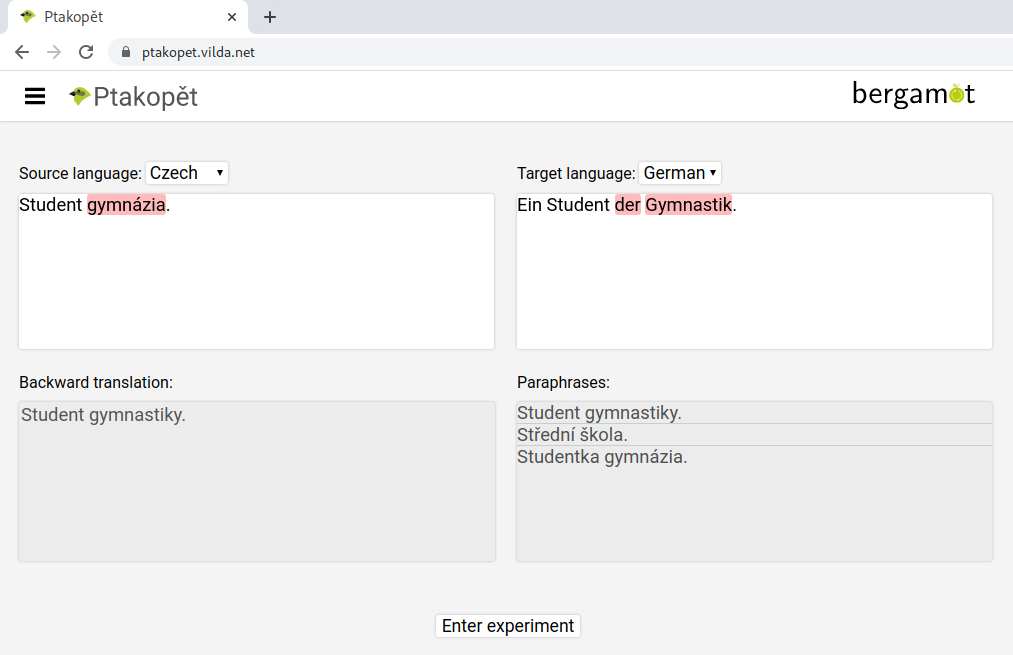
\includegraphics[width=\textwidth]{img/usage/usage-1.png}
  \caption{\label{fig:usage-1} \ptakopet{} is used to translate a simple Czech noun phrase to German. QE highlights parts of both source and target, that were translated incorrectly.}
\end{figure}

In \cref{fig:usage-1} it is seen, that the source was mistranslated by the red highlighting (on both source and target), but also by the backward translation. Paraphrases (or source variations) are displayed in the second to last block. In the case of simple noun phrases, they are irrelevant, but they are useful for more complex inputs, as shown in \cref{fig:usage-2}. In those cases, the user might want to reformulate (mostly simplify) specific parts of their input, so that the MT system can produce a better translation. 

Unfortunately, we found the quality estimation not to be reliable enough. It usually works only with concise sentences or simple noun phrases. This can be seen when comparing the highlighting in \cref{fig:usage-1} and \cref{fig:usage-2}.

The translation can be then also edited. A common error of MT systems is that they try to translate named entities. This is easy to recognize even in languages the user is not proficient in. They may then choose to fix this error in the translation textarea and check that all went well in the backward translation block. Typing anything in the source textarea would then rewrite these manual changes.

The backend for each service can be selected in the settings burger menu, hidden behind the burger icon in the top left corner in \cref{fig:usage-1}. The expanded settings menu is shown in \cref{fig:usage-settings} in the last block. Changing any language or backend selection causes a cascade so that relevant information is recomputed and showed. Pending requests to a specific backend are signalized by a loading indicator next to every module block.

\begin{figure}[ht]
  \centering
  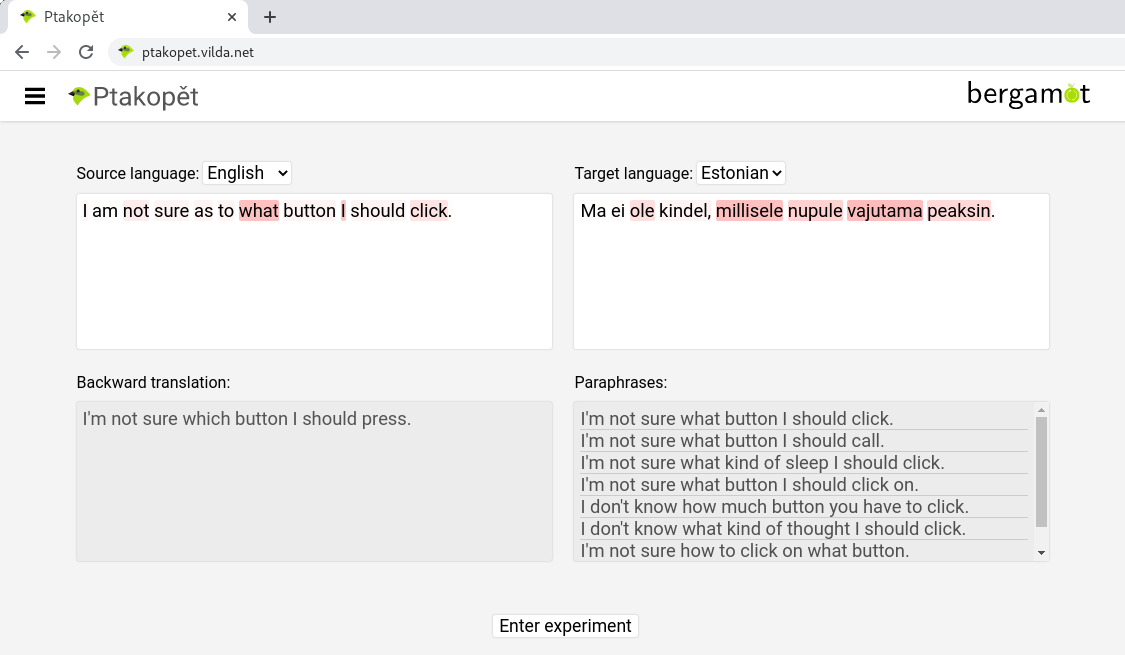
\includegraphics[width=\textwidth]{img/usage/usage-2.png}
  \caption{\label{fig:usage-2} \ptakopet{} is used to translate a complex English sentence to Estonian. User may opt to reformulate the input according to the paraphrases suggestions.}
\end{figure}

\begin{figure}[ht]
  \centering
  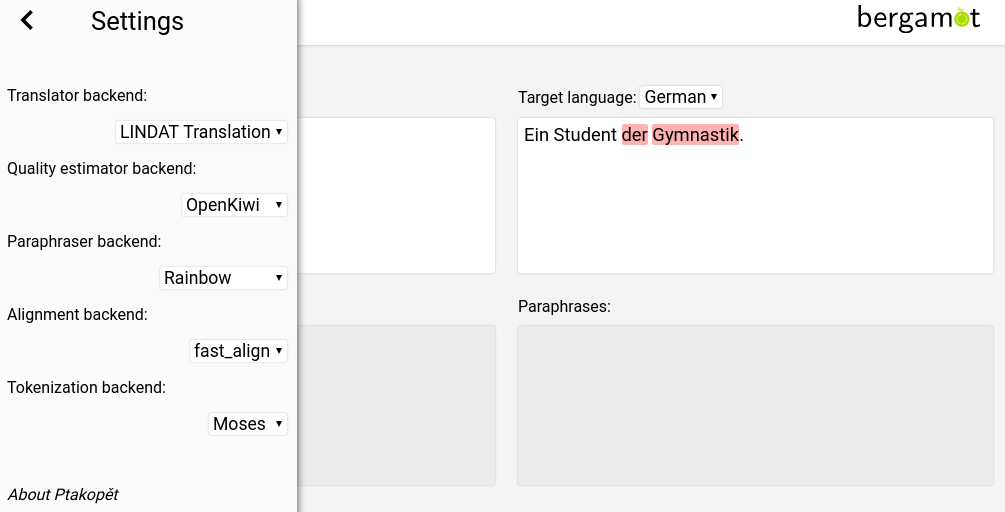
\includegraphics[width=\textwidth]{img/usage/usage-settings.png}
  \caption{\label{fig:usage-settings} Expanded settings burger menu in \ptakopet{}, which allows the users to change service backends.}
\end{figure}

\section{Settings overview}
\label{sec:usage-settings}

Backend settings are freely accessible, even though we do not expect most users to interact with them. Some particular settings are not intended to be used for outbound translation but are included either as placeholders or for debugging or presentation purposes. In this section, we aim to give a brief overview of their respective roles and origins. Backends, which were not created or setup by the author of this thesis, are explicitly mentioned.

An exclamation mark is shown next to the specific module in case the selected backend is incompatible with a given language pair. This warning is seen in \cref{fig:usage-mobile}.

\subsection*{Translator}

The main translator backend is \backendname{LINDAT Translation} \citep{popel-en-cs}, which provides translations between Czech, English, French and German. \backendname{Strong EN-CS} is just a shadow copy of this backend. Due to a collaboration with Tartu on the Bergamot project, we also added English$\leftrightarrow$Estonian backend \backendname{Neurotõlge}\footnotehref{https://neurotolge.ee/}{neurotolge.ee} and \backendname{Avg EN-ET}. For future experiments, we also added \backendname{Weak EN-CS} and \backendname{Strong EN-CS} for English$\leftrightarrow$Czech translation at various quality. There are also two placeholder backends, which evaluate client-side. \backendname{Identity} only copies the input and \backendname{None/Manual} does nothing so that the user can input their own texts without being interrupted. All of the non-local backends are not part of the work on this thesis.

\subsection*{Quality Estimation}

Our instances of \backendname{OpenKiwi} and \backendname{DeepQuest} backends support Czech$\rightarrow$German and English$\rightarrow$German quality estimation. The running instance of \backendname{QuEst++} supports English$\rightarrow$Czech quality estimation but is of very low quality. Collaborators from the Bergamot project who specialize in quality estimation provided two backends \backendname{Sheffield EN-ET} and \backendname{Sheffield EN-CS}. For presentation purposes, the QE values can be inputted manually by selecting the \backendname{Manual} backend. It can also be set to \backendname{Random}, which assigns each target word a random value between 0 and 1. This fake backend is good for analyzing alignment because one can then easily see what the words map to. The highlighting can be turned off by selecting \backendname{None}.

\subsection*{Paraphraser}

The first paraphraser is \backendname{LINDAT Mock}, which relies on round-trip translation with LINDAT Translation. It is extremely unoptimized and is there only for testing purposes. The second paraphraser backend, \backendname{Rainbow}, works on a similar principle but is more elaborate and faster. This backend is a transformer-based and is the work of Matúš Žilinec.\footnotehref{https://github.com/mzilinec/paraphrase-server}{github.com/mzilinec/paraphrase-server} The paraphraser module can also be turned off by selecting \backendname{None} as the paraphraser backend.

\subsection*{Alignment}

Alignment requests for most languages are by default relayed to \backendname{fast\_align Ubuntu} on server-side. There also exists a special backend \backendname{fast\_align Michal} which was setup by a colleague Michal Novák for future experiments with \ptakopet{} on English-Estonian and English-Czech language pairs. The alignment can also be evaluated locally by \backendname{Diagonal} placeholder backends, which for sentences of $M$ and $N$ tokens generates alignment $\{(i, j): 0 \le i \le M, 0 \le j \le N\}$. The \backendname{None} turns off the alignment altogether.

\subsection*{Tokenization}

The \backendname{Moses} tokenizer is the main tokenization backend and is very robust. There are two alternatives, which evaluate client-side. The first one, \backendname{Spaces}, is just splitting by single spaces, while the second one, \backendname{Local}, uses a more complex tokenization scheme.

\section{Miscellaneous}

\subsection*{Omnibox OpenSearch}
Google services and most notably Google Translate use omnibox OpenSearch to improve the user experience. This was also implemented in \ptakopet{}, so instead of having to go to the web page and then start typing the source text, it can be typed in the address bar after pressing the \texttt{TAB} key. The web page is then loaded and the input pasted in the input textarea.

This makes it more convenient for using \ptakopet{} to quickly translate pieces of texts. An example omnibox input and the result is shown in \cref{fig:usage-omnibox}.

\begin{figure}[ht]
  \centering
  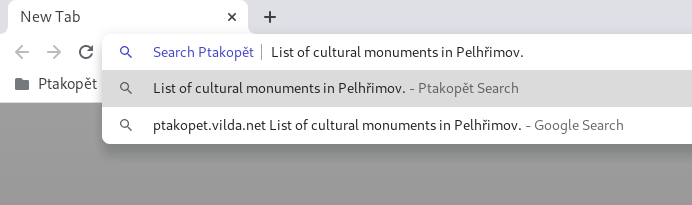
\includegraphics[width=\textwidth]{img/usage/omnibox-opensearch-1.png}
  \text{}\vspace{0.5cm}
  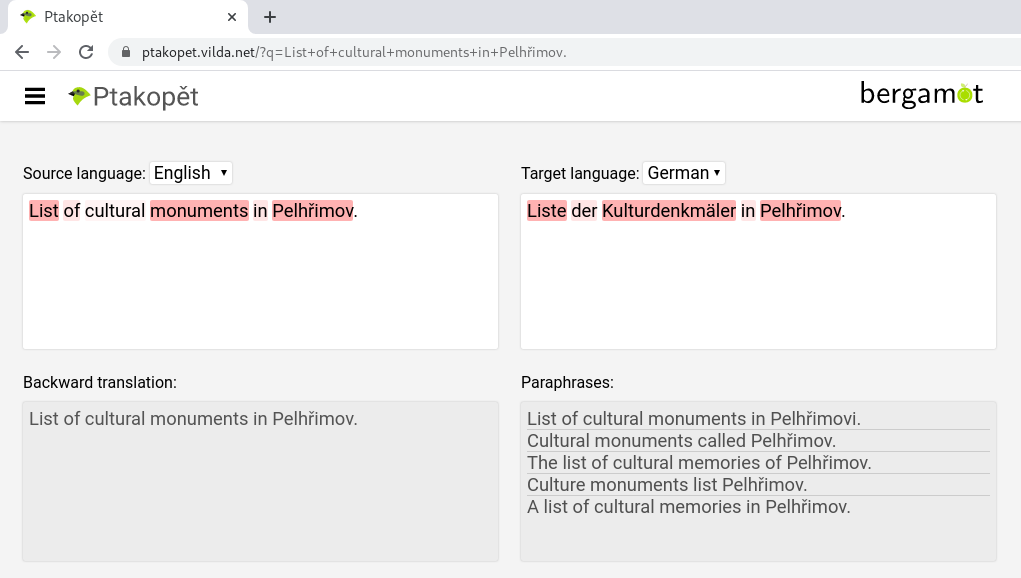
\includegraphics[width=\textwidth]{img/usage/omnibox-opensearch-2.png}
  \caption{\label{fig:usage-omnibox} Example usage of omnibox OpenSearch input. The text appears in the main input textarea once the user hits \texttt{ENTER}. The default language and backends settings are used.}
\end{figure}

\pagebreak

\subsection*{URL parameters}

\ptakopet{} also supports other URL GET parameters:
\begin{itemize}
    \item \texttt{userID} logs the user to the experiment by the supplied userID value. The experiment is discussed in \cref{sec:experiment_def} and \cref{chp:experiment}.
    \item \texttt{q} pastes the text query into the input box. This is to support the omnibox OpenSeach functionality.
    \item \texttt{p} sets a given settings profile to other than \texttt{default}, e.g. \texttt{pilot}, \texttt{edin}, \texttt{csen} or \texttt{sao}. This is helpful when one wishes to provide a quick link with all settings prepared. These exact settings profiles were used for different presentation purposes.
    \item \texttt{source} sends this extra value to the start log.
    \item \texttt{test} used for testing, described in \cref{subsubsec:implementation_testing}.
\end{itemize}

The redirect URL for profile \texttt{pilot} with the user \texttt{testuser} and source information \texttt{online-ad} can then look like:

\texttt{ptakopet.vilda.net/?p=pilot\&userID=testuser\&source=online-ad}

\subsection*{Error masking in backtranslation} \label{sec:error_masking}

When using the same data for both forward and backward MT, an error can be introduced in forward translation but removed in the backward translation. After experimenting with \ptakopet{} we found several examples described in \cref{fig:error_masking_example}. All can be tested in the live system using the \backendname{LINDAT Translation} backend.

\begin{figure}[ht]
    \begin{align*}
        \text{svírá úhel} \hspace{1cm} &\xrightarrow{\text{de}} &\text{Er schließt den Winkel.} \hspace{1cm} &\xrightarrow{\text{cs}} &\text{Zavírá úhel.} \\
        \text{svírá úhel} \hspace{1cm} &\xrightarrow{\text{fr}} &\text{Sait l'angle} \hspace{1cm}  &\xrightarrow{\text{cs}} &\text{Zná úhel} \\
        \text{svírá úhel} \hspace{1cm} &\xrightarrow{\text{en}} &\text{grips the angle} \hspace{1cm}  &\xrightarrow{\text{cs}} &\text{svírá úhel} \\
    \end{align*}
    \caption{\label{fig:error_masking_example} Example of error masking in backward translation in English MT compared to German and French MT in which the error is revealed.}
\end{figure}

The German and French MT in \cref{fig:error_masking_example} introduced an error in forward translation, but the backward translation was accurate and thus, the user could recognize this and reformulate the input. However, in the case of the English machine translation, an error is still introduced in the forward translation but the backward translation removes this error. The backward translation could, in fact, be accurate and this masking could be a result of sense ambiguity of the word ``svírat''. Nevertheless, the user could then get a false sense of a correct translation, which is undesirable.


\subsection*{Platforms}

\begin{figure}[ht]
  \centering
  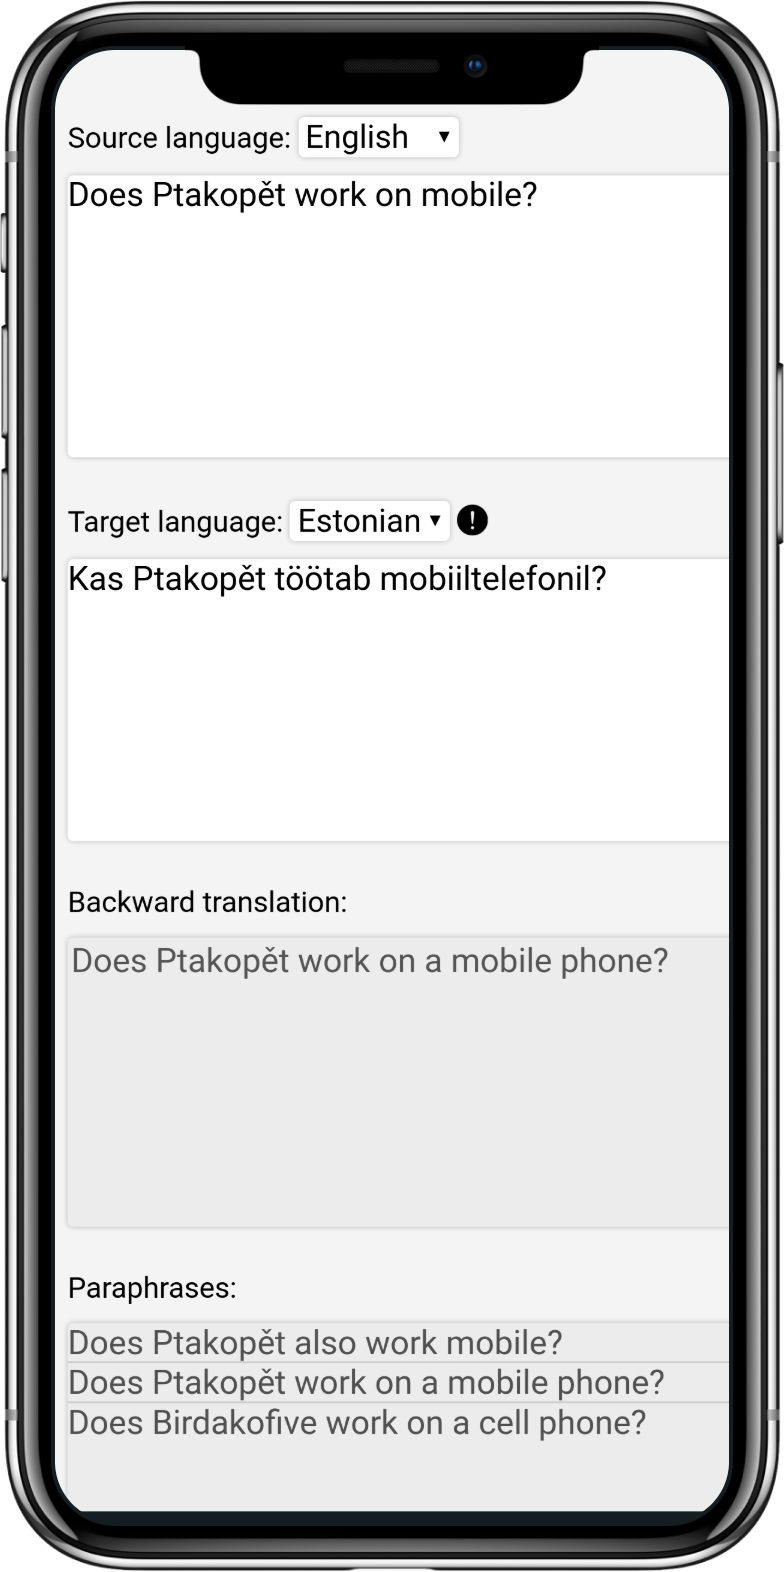
\includegraphics[width=0.45\textwidth]{img/usage/usage-mobile-mockup.png}
  \caption{\label{fig:usage-mobile} Mockup of \ptakopet{} in single column layout on phone.}
\end{figure}
% https://dimmy.club/phones/iphone-x

\ptakopet{} was tested to run properly on Edge 80, Chrome 83, Firefox 75 and Opera 66.

We wanted \ptakopet{} to be accessible from as many devices as possible and not just desktops. The frontend was designed to adapt to almost any screen size, most notably mobile. The layout is then changed to a single column, as shown in \cref{fig:usage-mobile}.

We found \ptakopet{} to be very usable on mobile. The only issue was that occasionally deleting of already written text could not be done by holding the backspace key. This is due to the highlighter dependency. \ptakopet{} was also tested to work without any issues on very computationally limited device, namely Samsung Smart TV with Tizen OS.